\chapter{Estudio sobre el acero F138}\label{C:F138}
\graphicspath{{./figs/04_F138/}}

En este capítulo se estudia la microestructura del acero inoxidable F138.
Este acero es de tipo austenítico, es decir que tiene una estructura FCC y tiene una composición que puede verse en la Tabla \ref{tab:F138Comp}.
Se caracteriza por tener una elevada resistencia a la corrosión, lo que lo hace útil para aplicaciones biomédicas y en energía nuclear.
Según el estudio realizado por Scheriau et al \cite{Scheriau2011} la deformación plástica severa se caracteriza por dos modos de deformación principales maclado mecánico (con maclas de 10-20\,nm de ancho) y bandas de corte submicrométricas que dividen el material en bloques micrométricos de láminas de maclas.
Liu et al. \cite{Liu2010} observaron una respuesta similar en un acero 316L sometido a deformación plástica dinámica, donde la estructura final evolucionó hacia una configuración de granos micrométricos de austenita junto con maclas nanométricas, confiriéndole al material una tensión de fluencia casi cinco veces mayor que aquella correspondiente a la estructura inicial de granos grandes.

\begin{table}[!htb]
\centering
\caption{Composición del acero inoxidable F138 (\% en peso dado por el fabricante)}
\label{tab:F138Comp}
\begin{tabular}{|c|c|c|c|c|c|c|c|c|c|c|}
\hline
\rowcolor[HTML]{BBDAFF} 
\textbf{Fe} & \textbf{Cr} & \textbf{Ni} & \textbf{Mo} & \textbf{Mn} & \textbf{Si} & \textbf{Cu} & \textbf{N} & \textbf{C} & \textbf{P} & \textbf{S} \\ \hline
          &    17.33  &   14.31   &   2.79    &   1.79    &  0.30     &   0.09    &   0.079   &  0.015    &   0.022   &   0.002   \\ \hline
\end{tabular}
\end{table}

El 2.5\% de Mo agregado mejora la resistencia a la corrosión, y al encontrarse en solución sólida contribuye a reducir la movilidad de las dislocaciones \cite{Chowdhury2005}.

El grupo de trabajo al que pertenece el autor de esta tesis tiene antecedentes de trabajo, tanto en muestras laminadas como en muestras deformadas por medio de la técnica de \textit{Deformación de Igual Canal Angular} (ECAE, por sus siglas en inglés)\cite{Devincentis2015PhD,Devincentis2017}, aunque los estudios realizados se concentraron previamente en mediciones de EBSD y en estudios de ancho de pico a través de los métodos de Williamson-Hall y CMWP.
En la Sec. \ref{S:F138Nati} se realiza un repaso de los principales resultados que se tienen sobre este material, mientras que en la Sec. \ref{S:F138LANG} se aplica el método de Langford a muestras de acero F138 laminadas hasta lograr una reducción de la reducción transversal del 70\,\%.

\nomenclature{ECAE}{Equal Angle Angular Extrusion, Deformación de Igual Canal Angular}
\section{Estado del arte en el estudio de la microestructura}\label{S:F138Nati}
En esta sección se presentan los resultados previos obtenidos en el grupo de investigación al que pertenece el autor de esta tesis. Los mismos incluyen mediciones de EBSD y estudios de ancho de pico empleando los métodos de Williamson-Hall y CMWP, y se encuentran publicados en \cite{Devincentis2015PhD,Devincentis2017}.

En la Fig. \ref{fig:F138PF} se encuentran las FP recalculadas a partir de las mediciones de textura realizadas en sincrotrón, donde pueden apreciarse la presencia de la fibra \{110\}\textless uvw\textgreater. 
Las FP de la Fig. \ref{fig:F138PF} provienen de la FDO que se observa en la Fig. \ref{fig:F138ODF}, donde se puede ver más claramente la fibra \{110\}\textless uvw\textgreater, en la sección $\varphi_2 \ = \ 0$\,$^{\circ}$, a lo largo de la coordenada $\Phi \ = \ 45$\,$^{\circ}$.

\begin{figure}[!htb]
  \centering
  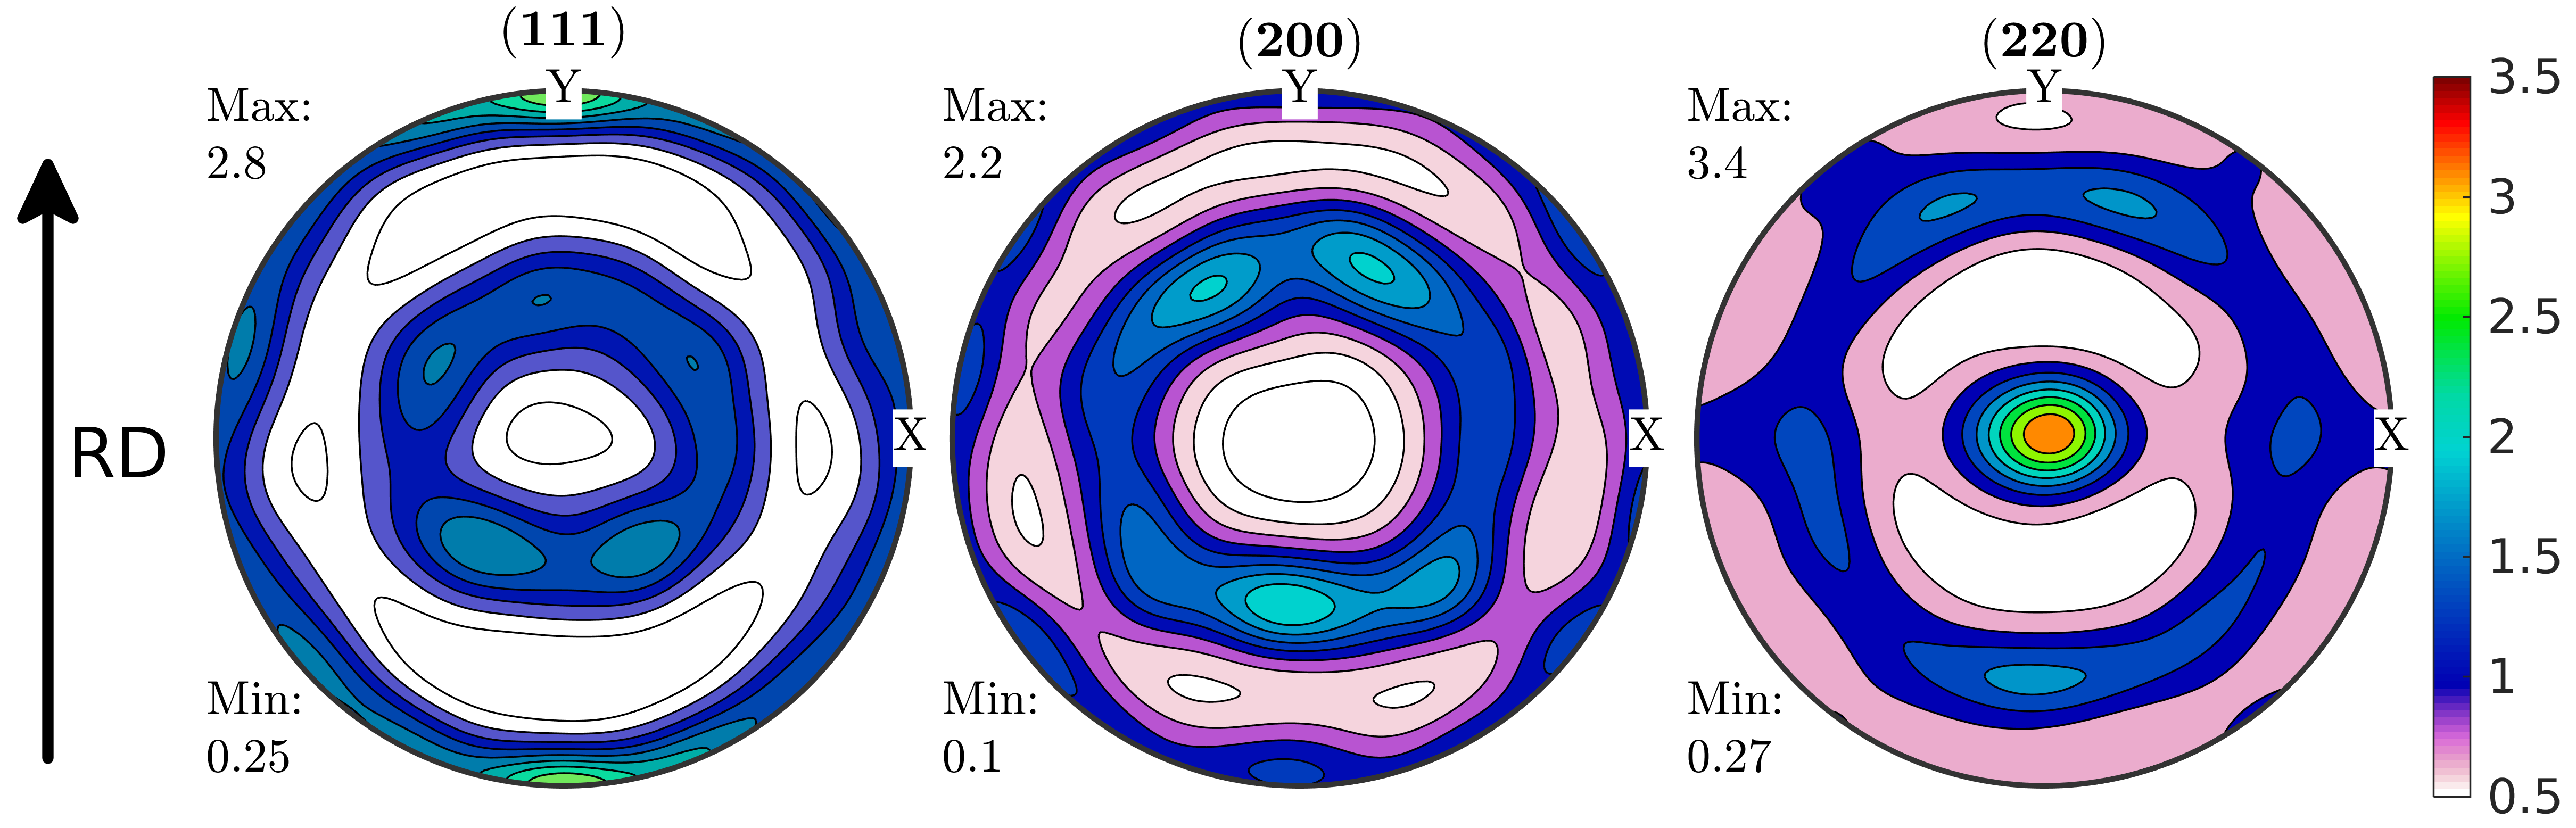
\includegraphics[width=\textwidth]{F138_Rec_RD}
  \caption{Textura F138 con sincrotron}
  \label{fig:F138PF}
\end{figure}

Observando la sección $\varphi_2 \ = \ 0$\,$^{\circ}$ de la FDO también puede apreciarse que la fibra no tienen intensidad uniforme, sino que la misma incrementa su intensidad en la componente  G/B(T) (\{110\}\textless 111\textgreater). 
La componente Goss (\{110\}\textless 001\textgreater), que fue observada claramente al estudiar la textura empleando rayos X de laboratorio con geometría de reflexión, tiene aquí una intensidad próxima a la del resto de la fibra.
Esta diferencia fue atribuida a heterogeneidades en la textura del material laminado a lo largo de la dirección ND, apreciables sólo en lo experimentos de transmisión, pero no en los de reflexión, y que tienen el efecto de suavizar la componente orientada a lo largo de ND.

\begin{figure}[!htb]
  \centering
  \includegraphics[width=\textwidth]{F138_odf}
  \caption{ODF del F138}
  \label{fig:F138ODF}
\end{figure}

En la sección $\varphi_2 \ = \ 45$\,$^{\circ}$ puede observarse el mismo comportamiento que para $\varphi_2 \ = \ 0$\,$^{\circ}$, pero además puede apreciarse la presencia de la componente Dillamore en las coordenadas $(\varphi_1, \Phi, \varphi_2) \ = \ (90, 30, 45)$\,$^{\circ}$.
La presencia de estas componentes es esperable en materiales laminados.
La anisotropía en la dirección cristalina \{220\} se asocia a la baja energía de falla de apilamiento en aceros\cite{Sathiaraj2015,Saleh2012}, aunque los análisis realizados empleando el método CMWP en distintas direcciones indican que el laminado de 70\,\% fue poco efectivo en introducir maclas, sobre todo cuando se compara con la cantidad introducida al deformar la muestra por ECAE.
Para tener como referencia, las estimaciones de CMWP indicaron que la proporción de maclas está por debajo de las 3 fallas de apilamiento/$\mu$m, lo cual sugiere además que la contribución de las fallas de apilamiento al ensanchamiento de los picos de difracción puede dejarse de lado.
Esto último es particularmente importante teniendo en cuenta que en la próxima sección se estudiará en ensanchamiento de los picos de difracción empleando el método de Langford, ya que como se explicó en la Sec. \ref{SS:Twin} la contribución de las fallas de apilamiento no se puede introducir sencillamente en dicho modelo.

Los estudios realizados aplicando los métodos CMWP y Williamson-Hall ambos revelaron tamaños de dominio del orden de los 50 nm para las tres direcciones de muestra, con valores algo mayores para los tamaños de dominios observados en la dirección de laminado, RD.
La densidad de dislocaciones obtenida fue del orden de 1 $\times$ 10$^{16}$\,m$^{-2}$ para las direcciones RD y TD, y del orden de 1.5 $\times$ 10$^{16}$\,m$^{-2}$ para la dirección ND.
Esta discrepancia recuerda los discutido en el Cap. \ref{C:IF}, donde se mencionó que la densidad de dislocaciones debe ser una cantidad independiente de la dirección de la muestra que se esté observando.

En \cite{Devincentis2017} se observa además que la anisotropía observada en ND tiene probablemente su raíz en la familia de planos \{220\}.
En la Fig. \ref{fig:F138NatiWHvsEquipos} pueden observarse las curvas de Williamson-Hall obtenidas a partir de las mediciones realizadas con un difractómetro X'Pert de laboratorio (a)  y las realizadas en DESY (b).
En ambos casos puede apreciarse que el ancho de pico, corregido con su respectivo factor de contraste, se encuentra claramente alejado de la curva definido por los ensanchamientos medidos en el resto de los picos.
Es más, también se observó que esta tendencia se observa sólo en los difractogramas medidos a los largo de ND, mientras que las curvas de Williamson-Hall medidas a lo largo de RD y TD son suaves y continuas.

\begin{figure}[!htb]
  \centering
  \includegraphics[width=\textwidth]{F138_WH_Equipos}
  \caption{Williamson Modificado para distintos equipos donde se ve el problema del pico 220. Sacado de \cite{Devincentis2017}.}
  \label{fig:F138NatiWHvsEquipos}
\end{figure}

Desde luego, este tipo de anisotropía llevó a estudiar el efecto de la textura en el cálculo de los factores de contraste calculados para las muestras laminadas, cuyos valores pueden apreciarse en la Fig. \ref{fig:F138NatiContrast}.
Puede verse que los factores de contraste obtenidos para las tres direcciones son relativamente similares, aunque se observa una dispersión levemente mayor para los planos \{220\}, en particular en la dirección ND, lo cual es consistente con lo discutido en el Cap. \ref{C:IF}, básicamente que existe cierta anisotropía en la acumulación de defectos que no puede ser explicada completamente a partir del modelo del factor de contraste, lo que implicaría que distintas poblaciones cristalinas han desarrollado microestructuras claramente diferentes.

\begin{figure}[!htb]
  \centering
  \includegraphics[width=0.7\textwidth]{F138_WH_DESY_Contrast}
  \caption{Factores de contraste para las tres direcciones con los anchos medidos en DESY. Sacado de \cite{Devincentis2017}.}
  \label{fig:F138NatiContrast}
\end{figure}

En este sentido parecería que los cristales orientados según la dirección \textless220\textgreater$\parallel$ND exhiben un ensanchamiento claramente inferior al resto de las componentes de textura del material, lo que implicaría que estos cristales han acumulado una cantidad de defectos notablemente menor que el resto.
Esto puede implicar que los cristales con dirección \textless220\textgreater$\parallel$ND tienen dominios más grandes y/o han acumulado menos dislocaciones.

Los resultados obtenidos fueron verificados empleando microscopía electrónica de barrido, por medio de la técnica de EBSD.
En particular, dado que la textura está marcada por presencia de la fibra \{110\}\textless uvw\textgreater, y que la mayor anisotropía se observó en los planos \{220\}, se realizó un estudio similar al descripto en el Cap. \ref{C:IF}.

En la Fig. \ref{fig:F138EBSDNati} se aprecian dos de los principales resultados de este estudio, el tamaño de grano para distintas direcciones de muestra (Fig. \ref{fig:F138EBSDNati}-a) y la distribución de GNDs (Fig. \ref{fig:F138EBSDNati}-b), para las diferentes particiones de interés, definidas en función de la orientación de la familia de planos \{220\} respecto de los ejes principales de la muestra.

\begin{figure}[!htb]
  \centering
  \includegraphics[width=\textwidth]{F138_EBSD_SizeyGNDvsDirection}
  \caption{Tamaño de dominio (longitud de intercepción) y GND según dirección cristalina. Imágenes obtenidas de \cite{Devincentis2017}.}
  \label{fig:F138EBSDNati}
\end{figure}

Los resultados de EBSD son consistentes con lo observado a través de los experimentos de XRD, ya que el tamaño de grano de los cristales con dirección \textless220\textgreater$\parallel$ND es notablemente mayor que la de los cristales de la partición complementaria, mientras que no se observa un cambio tan importante cuando se observa a la muestra en las direcciones TD y RD.
Adicionalmente, según lo mostrado en la distribución de GND de la Fig. \ref{fig:F138EBSDNati}-b, los cristales con orientación \textless220\textgreater$\parallel$ND tienen en promedio menos dislocaciones que los que no se encuentran con la dirección \{220\} paralela a ND.
Vale la pena notar que la densidad de dislocaciones medida por EBSD da un valor que es aproximadamente dos órdenes de magnitud inferior a lo estimado por medio de Williamson-Hall y CMWP.
Esto se debe a algo.

Las mediciones de EBSD también revelaron que la partición \textless220\textgreater$\nparallel$ND posee, a diferencia del resto de las particiones analizadas, una proporción importante de \textit{bordes de grano de alto ángulo} (HAGB, por sus siglas en inglés), lo que sugiere que se ha producido recristalización dinámica en el material, como consecuencia del laminado.
El hecho de que la recristalización haya ocurrido en una población cristalina particular sugiere a su vez que distintas poblaciones de cristales han acumulado una cantidad de energía muy diferente como consecuencia del laminado.
En \cite{Devincentis2015} lo autores observaron un comportamiento similar sobre el mismo material, aunque esta vez al ser sometido a 4 pasadas de ECAE.

Además, los HAGB se caracterizan por ser arreglos compactos con alta densidad de dislocaciones, en contraposición con los \textit{bordes de grano de bajo ángulo} (LAGB, por sus siglas en inglés), que tienden a acumular menos dislocaciones que además se encuentran menos correlacionadas.
En este sentido entonces, es razonable que los cristales cuyos planos \{220\} son paralelos a ND revelen menor número de dislocaciones que aquellos de la partición complementaria, y por lo tanto menor ensanchamiento, que aquellos cristales que no tengan ésta característica.

La fallas de apilamiento no son suficientes como para contribuir al ensanchamiento pero sí como para modificar la textura

\nomenclature{HAGB}{Siglas en inglés para Bordes de grano de alto ángulo (High Angle Grain Boundary).}
\nomenclature{LAGB}{Siglas en inglés para Bordes de grano de bajo ángulo (Low Angle Grain Boundary).}

\newpage
\section{Estudio de la microestructura por el método de Langford y figuras de polos generalizadas}\label{S:F138LANG}
Al observar las FDO Generalizadas de Tamaño de cristalita y deformación, Figs. \ref{fig:F138Size} y \ref{fig:F138Strain} respectivamente, puede verse un comportamiento similiar al observado en el acero libre de intersticiales (Cap. \ref{C:IF}) en donde ciertas componentes favorecidas por la textura tienen mayor tamaño de cristalita y acumulan menos deformación, lo que en este caso se traduce a una menor densidad de dislocaciones.
En este caso puede verse que es la componente Goss es la componente que ``más limpia'', mientras que en la componente G/B(T) se tienen dominios un poco más grandes, pero con menor cantidad de dislocaciones acumuladas.
\begin{figure}[!htb]
  \centering
  \includegraphics[width=\textwidth]{F138_size_odf}
  \caption{Size ODF F138}
  \label{fig:F138Size}
\end{figure}

\begin{figure}[!htb]
  \centering
  \includegraphics[width=\textwidth]{F138_strain_odf}
  \caption{Strain ODF}
  \label{fig:F138Strain}
\end{figure}




\newpage
\section{Discusión de resultados}\label{S:F138Dis}
\newpage
\section{Conclusiones}\label{S:F138Conclusiones}
